\section*{Introduction}
\addcontentsline{toc}{section}{Introduction}

The transfer matrix method provides a powerful tool to study systems built from a repeated, macroscopic structure.  In this paper, I will demonstrate how to apply the transfer matrix method to entirely capture the bulk and surface screening response of superlattices.  In particular, we will arrive at an analytical expression for the electronic density response function,
\begin{equation}
    \label{Fourier density response def}
    \chi(q,\omega):=\chi(q,q';\omega)_{q=q'}
    :=
    \lb\frac{1}{\vol}\int d^3 r d^3 r' e^{iq\cdot r} e^{-i q'\cdot r'}\chi(r,r';\omega)\rb_{q=q'}
    \,\,\,,
\end{equation}
where $q$ is the wavevector and $\omega$ is the frequency of the screening response.  The quantity in \eqref{Fourier density response def} warrants study as it governs density-density scattering probes of the superlattice via the fluctuation-dissipation theorem.

In what follows, ``superlattice" refers to a system with translation-invariance along the planar directions (those perpendicular to the superlattice dimension)\footnote{This assumption can be relaxed to the discrete translation symmetry of a crystalline solid, so long as the ``long wavelength limit'' is appropriately redefined.} and discrete translation symmetry in the layering direction.  In particular, I'll focus on the geometry in Fig. \ref{figure: superlattice geometry}, where dielectric regions are separated by regularly-spaced conducting planes.\footnote{More complicated bi-layer, tri-layer, or n-layer systems are more or less amenable to the same analysis, as considered in \cite{Cottam1993, Cottam2004}.}  I will utilize an electrostatic framework, working in the non-relativistic and non-retarded limit governed by electric potentials and charge densities.  The subseqeuent electrostatic analysis roughly applies in the limit $q^2\gg \omega^2/c^2$, where $q$ and $\omega$ are the wavevector and frequency of excitations within this framework, respectively.

\begin{figure}
    \centering
    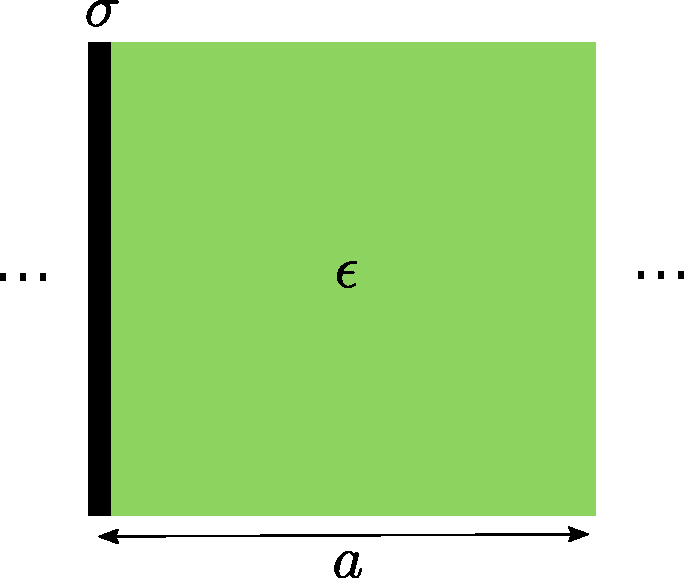
\includegraphics[width=\columnwidth]{figures/superlattice-geometry.pdf}
    \caption{
    {\bf TODO} -- finish caption.
    }
    \label{figure: superlattice geometry}
\end{figure}

